\documentclass[11pt]{article}
\usepackage{amsmath}
\usepackage{amssymb}
\usepackage{tikz}
%\usetikzlibrary{calc}
%\usetikzlibrary{trees}
\usetikzlibrary{positioning}
\usepackage{hyperref}
\usepackage{graphicx}
\graphicspath{ {../../chap08/} }
\usepackage[top=0.75in, bottom=0.75in, left=0.75in, right=0.75in]{geometry}
\newcommand*{\Scale}[2][4]{\scalebox{#1}{\ensuremath{#2}}}%
\usepackage[shortlabels]{enumitem}
\usepackage[most]{tcolorbox}
\definecolor{bg}{RGB}{255,249,227}
% \usepackage{showframe}
\usepackage{caption}
\usepackage{fdsymbol}


%\title{\vspace{-10ex}HANDOUT Math 208 Week 07}
%\date{\vspace{-10ex}}


\begin{document}
	\Large Counting into Boxes
	\normalsize


%\begin{tikzpicture}
%	\draw[black, thick] (-1,0) -- (6,0);
%	\draw[black, thick] (0,-1) -- (0,6);
%	\draw[blue, thick] (0,2) -- (2,0);
%	\draw[red, thick](0,4) -- (1,0);
%	\node at (2.5,-0.5) {$x + y = 2$};
%	\node at (1,4) {$4x + y = 4$};
%\end{tikzpicture}
%
%\begin{tikzpicture}
%	\draw[gray, thick] (-1,2) -- (2,-4);
%	\draw[gray, thick] (-1,-1) -- (2,2);
%	\filldraw[black] (0,0) circle (2pt) node[anchor=west] {Intersection point};
%\end{tikzpicture}
%
%\begin{tikzpicture}
%	\draw (-2,0) -- (2,0);
%	\filldraw [gray] (0,0) circle (2pt);
%	\draw (-2,-2) .. controls (0,0) .. (2,-2);
%	\draw (-2,2) .. controls (-1,0) and (1,0) .. (2,2);
%\end{tikzpicture}

%\begin{tikzpicture}
%	\filldraw[color=red!60, fill=red!5, very thick](-1,0) circle (1.5);
%	\fill[blue!50] (2.5,0) ellipse (1.5 and 0.5);
%	\draw[ultra thick, ->] (6.5,0) arc (0:220:1);
%\end{tikzpicture}
%
%\begin{tikzpicture}
%	\draw[blue, very thick] (0,0) rectangle (3,2);
%	\draw[orange, ultra thick] (4,0) -- (6,0) -- (5.7,2) -- cycle;
%\end{tikzpicture}

\begin{itemize}
	

\item Spell CAT.

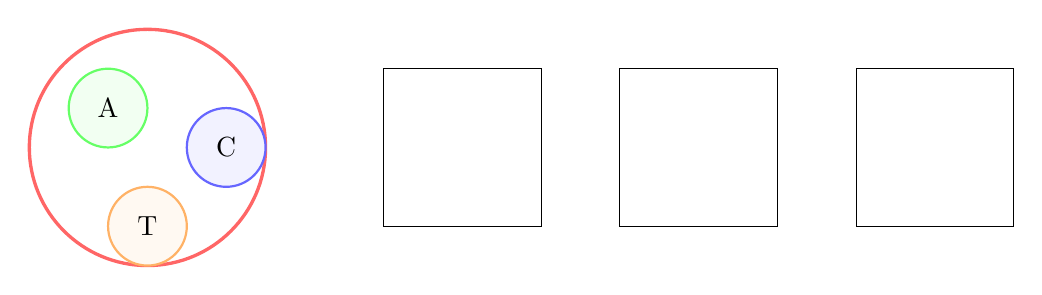
\begin{tikzpicture}
	\draw[color=red!60, very thick](-1,0) circle (1.5);
	\filldraw[color=green!60, fill=green!5, thick](-1.5,0.5) circle (0.5);
	\node at (-1.5,.5) {A};
	\filldraw[color=blue!60, fill=blue!5, thick](0,0) circle (0.5);
	\node at (0,0) {C};
	\filldraw[color=orange!60, fill=orange!5, thick](-1,-1) circle (0.5);
	\node at (-1,-1) {T};
	
	\draw (2,-1) rectangle (4,1);
	\draw (5,-1) rectangle (7,1);
	\draw (8,-1) rectangle (10,1);
\end{tikzpicture}
%\\\\
%\vspace{1cm}
%\begin{tikzpicture}
%	\draw (0,0) rectangle (2,2);
%	\draw (3,0) rectangle (5,2);
%	\draw (6,0) rectangle (8,2);
%%	\draw (6,0) rectangle (2,2);
%\end{tikzpicture}
\\\\
Q: How many different ways can you put the 3 letters into the 3 boxes such that you spell the word CAT?
\\\\
A: There is only 1 correct way to spell CAT, thus the answer is only 1 way.
\\\\
Q: How many different ways may the letters be arranged in the boxes?
\\\\
A: There are three possible letters for the first box. This leaves two possible letters for the second box and only one possible letter for the last box. Therefore $3*2*1 = 3! = 6$. These possibilities are:
$$S=\{ACT,ATC,CAT,CTA,TAC,TCA\}$$


\item Suppose that 6 people check their coats in a checkroom. If all claim checks are lost and the 6 coats are randomly returned, what is the probability that all the people will get their own coats back?

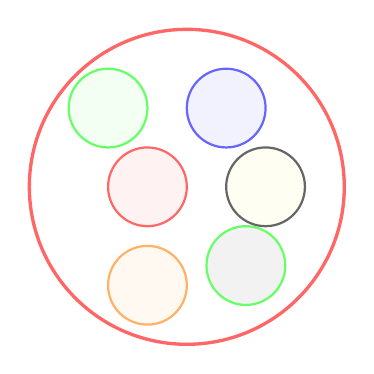
\begin{tikzpicture}
	\draw[color=red!60, very thick](-1,0) circle (2.0);
	\filldraw[color=green!60, fill=green!5, thick](-2,1) circle (0.5);
	\filldraw[color=blue!60, fill=blue!5, thick](-.5,1) circle (0.5);
	\filldraw[color=orange!60, fill=orange!5, thick](-1.5,-1.25) circle (0.5);
	\filldraw[color=red!60, fill=red!5, thick](-1.5,0) circle (0.5);
	\filldraw[color=green!60, fill=black!5, thick](-.25,-1) circle (0.5);
%	\filldraw[color=purple!60, fill=purple!5, thick](1,0) circle (0.5);
	\filldraw[color=black!60, fill=yellow!5, thick](0,0) circle (0.5);
\end{tikzpicture}



\begin{tikzpicture}
%	\filldraw[fill=blue!40!white, draw=black] (0,0) rectangle (4,4);
	\filldraw[color=green!60, fill=green!5, very thick] (0,0) rectangle (2,2);
	\filldraw[color=blue!60, fill=blue!5, very thick] (3,0) rectangle (5,2);
	\filldraw[color=orange!60, fill=orange!5, very thick] (6,0) rectangle (8,2);
	\filldraw[color=red!60, fill=red!5, very thick] (9,0) rectangle (11,2);
	\filldraw[color=green!60, fill=black!5, very thick] (12,0) rectangle (14,2);
	\filldraw[color=black!60, fill=yellow!5, very thick] (15,0) rectangle (17,2);
\end{tikzpicture}
\\\\
Q: How many different ways can you put the 6 coats into the 6 boxes such that the colors match?
\\\\
A: There is only 1 correct way to place each colored coat into the matching box, thus the answer is only 1 way.
\\\\
Q: How many different ways may the coats be placed into the boxes?
\\\\
A: There are 6 possible coats for the first box. This leaves 5 possible coats for the second box and then successively 4, then, 3, then 2, and finally 1. Therefore $6*5*4*3*2*1 = 6! =720$. These possibilities are too many to list.
 
\end{itemize}


%\begin{tikzpicture}[
%	roundnode/.style={circle, draw=green!60, fill=green!5, very thick, minimum size=7mm},
%	squarednode/.style={rectangle, draw=red!60, fill=red!5, very thick, minimum size=5mm},
%	]
%	%Nodes
%	\node[squarednode]      (maintopic)                              {2};
%	\node[roundnode]        (uppercircle)       [above=of maintopic] {1};
%	\node[squarednode]      (rightsquare)       [right=of maintopic] {3};
%	\node[roundnode]        (lowercircle)       [below=of maintopic] {4};
%	
%	%Lines
%	\draw[->] (uppercircle.south) -- (maintopic.north);
%	\draw[->] (maintopic.east) -- (rightsquare.west);
%	\draw[->] (rightsquare.south) .. controls +(down:7mm) and +(right:7mm) .. (lowercircle.east);
%\end{tikzpicture}




%
%\noindent\rule{\textwidth}{1pt}
%{\footnotesize Copyright (C) 2021 Garold Dalton --- Released under GNU General Public License v3.0}


\cleardoublepage


\end{document}
